% ==============================================================================
% 第五章: A4速查表 (打印用)
% ==============================================================================
\section{速查表}

\subsection{数值系统}

\begin{center}
\small
\begin{tabular}{|l|l|}
\hline
\textbf{概念} & \textbf{公式/规则} \\
\hline
$n$位无符号范围 & $[0, 2^n-1]$ \\
$n$位有符号范围 & $[-2^{n-1}, 2^{n-1}-1]$ \\
负数补码 & $-X \to 2^n - X$ \\
补码转值 & $-b_{n-1} \cdot 2^{n-1} + \sum b_i \cdot 2^i$ \\
符号扩展 & 复制MSB \\
溢出条件 & 正+正=负 或 负+负=正 \\
\hline
\end{tabular}
\end{center}

\subsection{卡诺图}

\begin{center}
\small
\begin{tabular}{|l|l|}
\hline
\textbf{规则} & \textbf{说明} \\
\hline
格雷码顺序 & 00, 01, 11, 10 \\
圈大小 & 必须是$2^n$ (1,2,4,8...) \\
环绕 & 左右/上下边可连 \\
四角 & 可组成一个圈 \\
Don't Care & 可当1扩大圈 \\
\hline
\end{tabular}
\end{center}

\textbf{4变量索引:}
\begin{center}
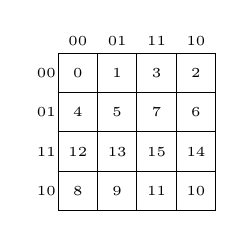
\begin{tikzpicture}[scale=0.5]
\draw (0,0) grid (4,4);
\node at (0.5, 4.3) {\tiny 00};
\node at (1.5, 4.3) {\tiny 01};
\node at (2.5, 4.3) {\tiny 11};
\node at (3.5, 4.3) {\tiny 10};
\node at (-0.3, 3.5) {\tiny 00};
\node at (-0.3, 2.5) {\tiny 01};
\node at (-0.3, 1.5) {\tiny 11};
\node at (-0.3, 0.5) {\tiny 10};
\node at (0.5,3.5) {\tiny 0};
\node at (1.5,3.5) {\tiny 1};
\node at (2.5,3.5) {\tiny 3};
\node at (3.5,3.5) {\tiny 2};
\node at (0.5,2.5) {\tiny 4};
\node at (1.5,2.5) {\tiny 5};
\node at (2.5,2.5) {\tiny 7};
\node at (3.5,2.5) {\tiny 6};
\node at (0.5,1.5) {\tiny 12};
\node at (1.5,1.5) {\tiny 13};
\node at (2.5,1.5) {\tiny 15};
\node at (3.5,1.5) {\tiny 14};
\node at (0.5,0.5) {\tiny 8};
\node at (1.5,0.5) {\tiny 9};
\node at (2.5,0.5) {\tiny 11};
\node at (3.5,0.5) {\tiny 10};
\end{tikzpicture}
\end{center}

\subsection{RS锁存器}

\begin{center}
\small
\begin{tabular}{|cc|c|l|}
\hline
S & R & Q$_{next}$ & 说明 \\
\hline
0 & 0 & Q & 保持 \\
0 & 1 & 0 & 复位 \\
1 & 0 & 1 & 置位 \\
1 & 1 & ? & 禁止 \\
\hline
\end{tabular}
\end{center}

特征方程: $Q_{next} = S + \bar{R}Q$

\subsection{香农展开}

\begin{center}
\fbox{$F = x \cdot F_{x=1} + \bar{x} \cdot F_{x=0}$}
\end{center}

\textbf{步骤:}
\begin{enumerate}
\item 令$x=1$,计算$F_1$
\item 令$x=0$,计算$F_0$
\item 组合: $F = xF_1 + \bar{x}F_0$
\end{enumerate}

\subsection{流水线}

\textbf{5级:} IF $\to$ ID $\to$ EX $\to$ MEM $\to$ WB

\textbf{冲突类型:}
\begin{itemize}
\item RAW: 读后写 (最常见)
\item Forwarding: EX/MEM$\to$EX, MEM/WB$\to$EX
\item Load-Use: 必须Stall 1周期
\end{itemize}

\textbf{性能:}
\[
\text{CPI} = 1 + \text{Stall率}
\]
\[
\text{Speedup} = \frac{nk}{k+n-1} \to k
\]

\subsection{布尔代数}

\begin{center}
\small
\begin{tabular}{|l|l|}
\hline
德摩根 & $\overline{A+B}=\bar{A}\bar{B}$, $\overline{AB}=\bar{A}+\bar{B}$ \\
吸收律 & $A+AB=A$, $A(A+B)=A$ \\
异或 & $A \oplus B = A\bar{B}+\bar{A}B$ \\
补余 & $A+\bar{A}=1$, $A\bar{A}=0$ \\
\hline
\end{tabular}
\end{center}

\subsection{常用数值}

\begin{center}
\small
\begin{tabular}{|c|c||c|c|}
\hline
$2^n$ & 值 & $n$位max & 有符号 \\
\hline
$2^4$ & 16 & 15 & $\pm7$ \\
$2^8$ & 256 & 255 & $\pm127$ \\
$2^{10}$ & 1024 & 1023 & $\pm511$ \\
$2^{16}$ & 65536 & 65535 & $\pm32767$ \\
\hline
\end{tabular}
\end{center}

\vspace{6pt}
\begin{center}
\textbf{Good Luck!}\\
\small 2026-01-13 10:00 | KN-A-310
\end{center}
